% Options for packages loaded elsewhere
\PassOptionsToPackage{unicode}{hyperref}
\PassOptionsToPackage{hyphens}{url}
%
\documentclass[
]{article}
\usepackage{lmodern}
\usepackage{amssymb,amsmath}
\usepackage{ifxetex,ifluatex}
\ifnum 0\ifxetex 1\fi\ifluatex 1\fi=0 % if pdftex
  \usepackage[T1]{fontenc}
  \usepackage[utf8]{inputenc}
  \usepackage{textcomp} % provide euro and other symbols
\else % if luatex or xetex
  \usepackage{unicode-math}
  \defaultfontfeatures{Scale=MatchLowercase}
  \defaultfontfeatures[\rmfamily]{Ligatures=TeX,Scale=1}
\fi
% Use upquote if available, for straight quotes in verbatim environments
\IfFileExists{upquote.sty}{\usepackage{upquote}}{}
\IfFileExists{microtype.sty}{% use microtype if available
  \usepackage[]{microtype}
  \UseMicrotypeSet[protrusion]{basicmath} % disable protrusion for tt fonts
}{}
\makeatletter
\@ifundefined{KOMAClassName}{% if non-KOMA class
  \IfFileExists{parskip.sty}{%
    \usepackage{parskip}
  }{% else
    \setlength{\parindent}{0pt}
    \setlength{\parskip}{6pt plus 2pt minus 1pt}}
}{% if KOMA class
  \KOMAoptions{parskip=half}}
\makeatother
\usepackage{xcolor}
\IfFileExists{xurl.sty}{\usepackage{xurl}}{} % add URL line breaks if available
\IfFileExists{bookmark.sty}{\usepackage{bookmark}}{\usepackage{hyperref}}
\hypersetup{
  pdftitle={Final Project: Is My Commute Really a Nightmare?},
  pdfauthor={Cleo C. Falvey},
  hidelinks,
  pdfcreator={LaTeX via pandoc}}
\urlstyle{same} % disable monospaced font for URLs
\usepackage[margin=1in]{geometry}
\usepackage{longtable,booktabs}
% Correct order of tables after \paragraph or \subparagraph
\usepackage{etoolbox}
\makeatletter
\patchcmd\longtable{\par}{\if@noskipsec\mbox{}\fi\par}{}{}
\makeatother
% Allow footnotes in longtable head/foot
\IfFileExists{footnotehyper.sty}{\usepackage{footnotehyper}}{\usepackage{footnote}}
\makesavenoteenv{longtable}
\usepackage{graphicx,grffile}
\makeatletter
\def\maxwidth{\ifdim\Gin@nat@width>\linewidth\linewidth\else\Gin@nat@width\fi}
\def\maxheight{\ifdim\Gin@nat@height>\textheight\textheight\else\Gin@nat@height\fi}
\makeatother
% Scale images if necessary, so that they will not overflow the page
% margins by default, and it is still possible to overwrite the defaults
% using explicit options in \includegraphics[width, height, ...]{}
\setkeys{Gin}{width=\maxwidth,height=\maxheight,keepaspectratio}
% Set default figure placement to htbp
\makeatletter
\def\fps@figure{htbp}
\makeatother
\setlength{\emergencystretch}{3em} % prevent overfull lines
\providecommand{\tightlist}{%
  \setlength{\itemsep}{0pt}\setlength{\parskip}{0pt}}
\setcounter{secnumdepth}{-\maxdimen} % remove section numbering

\title{Final Project: Is My Commute \emph{Really} a Nightmare?}
\author{Cleo C. Falvey}
\date{5/15/2020}

\begin{document}
\maketitle

\hypertarget{introduction}{%
\section{Introduction}\label{introduction}}

Ever since coming to campus in Fall 2017, I have become obsessed with
timing my commute and seeing how long it takes to go to Brookline
Village to UMass Boston. This data may have a limited scope of
importance, because my own commute has little effect on others' lives.
However, it does provide a fascinating glimpse into the inner workings,
such as they are, of the MBTA.

This is a more in-depth followup to a previous post on my statistics
blog which can be found
\href{https://graphmyundergrad.rbind.io/2019/06/27/tracking-my-nightmarish-commute/}{here}.
Previous analyses have shown that commuting at rush hour took about five
minutes longer than not commuting at rush hour.

\begin{figure}
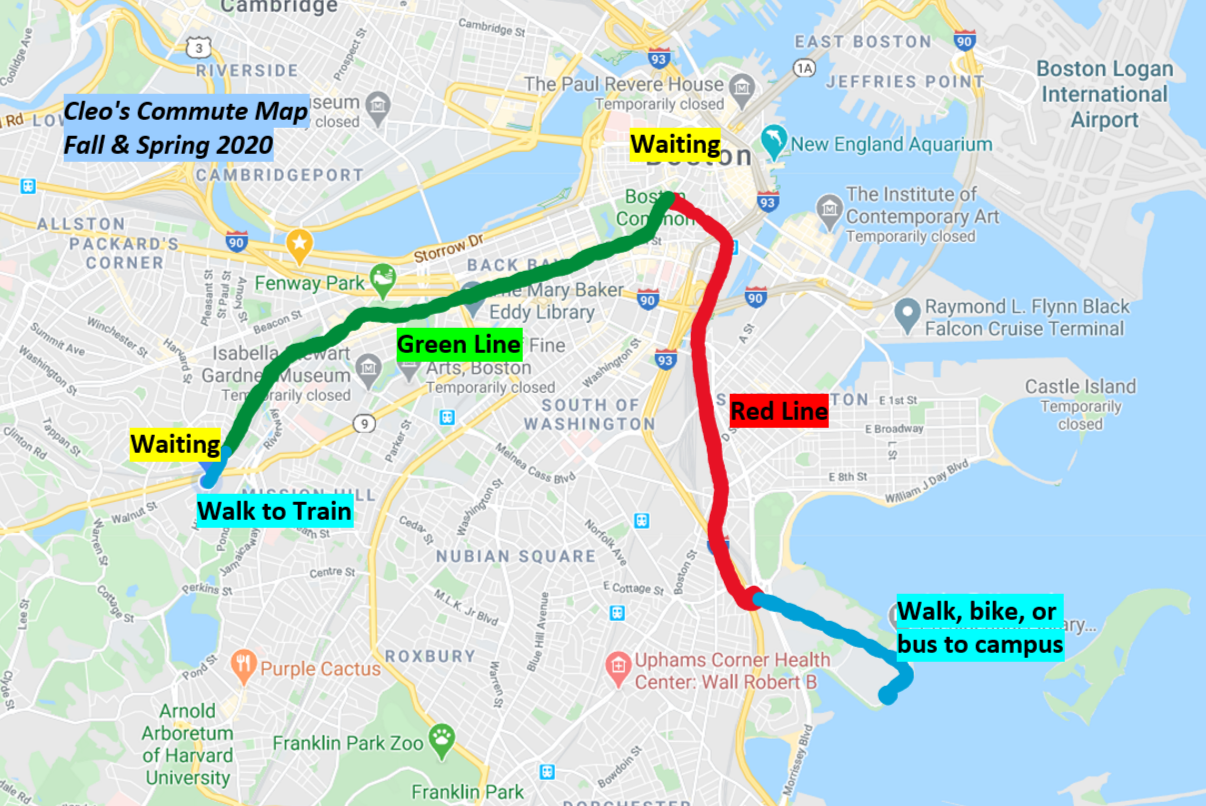
\includegraphics[width=1\linewidth]{commute_map} \caption{Cleo's Commute, Mapped Out}\label{fig:unnamed-chunk-2}
\end{figure}

\hypertarget{data}{%
\section{Data}\label{data}}

The data that I'm using has been painstakingly(!) collected across six
months of commuting to school in a convenience sampling method. The
structure of the dataset is as follows:

\begin{enumerate}
\def\labelenumi{\arabic{enumi}.}
\tightlist
\item
  Walking to my house from the train.
\item
  Waiting for the train (wait\_green).
\item
  Riding the green line from Brookline Village to Park Street
  (green\_line).
\item
  Waiting for the red line at Park Street (wait\_red).
\item
  Riding the red line from Park Street to JFK/UMass (red\_line).
\item
  Walking, biking, or taking the shuttle from JFK/UMass to campus
  (walk\_or\_bike).
\end{enumerate}

The process to go home occurs in reverse.

The methodology of collecting the data was that every time I commuted to
school or home on a weekday, I collected the time using a digital
wristwatch. I always rounded the time to the nearest minute for
simplicity's sake. I commuted in the same fashion in every day, and made
every attempt to minimize my commute time by running for the train at
top speed. I collected all of this data to the best of my ability,
although some random and systematic errors are present in the data.

\hypertarget{research-questions}{%
\section{Research Questions}\label{research-questions}}

\begin{enumerate}
\def\labelenumi{\arabic{enumi}.}
\tightlist
\item
  What is the average length of each section of the commute? This would
  involve calculating the sample mean and variance for each segment. I
  would also like to know whether these are normal or not, and present
  histograms and the results of Shapiro-Wilk tests for each segment.
\item
  If not normal, what probability distributions can I use to model each
  segment of my commute? Using the MLE and MoM, I hope to find
  probability distributions for each segment of the commute. I doubt
  they are all normally distributed, however; they might likely all be
  very right-skewed because although there is theoretically a minimum
  time needed to commute to school, due to delays, the commute could be
  hours long. Therefore, these longer commute times will pull out the
  durations, making the distributions abnormal. I would like to find the
  parameters for the probability distributions.
\item
  Is the difference between the length of the commute depending on the
  directionality (i.e., school to home versus home to school)? During my
  exploratory data analysis, I noticed that box plots created of
  distances had very different spreads. I would hope to test this with
  an F-test for variances between two populations.
\item
  What segments of the commute have the largest contribution to the
  overall length? This would deal with methods of correlation and linear
  modelling to see which parts of the commute have the largest impact to
  the total time.
\item
  How long can I expect my commute to be? Using the data, I would like
  to create confidence intervals for each segment.
\end{enumerate}

\hypertarget{question-1-how-long-are-my-commute-segments-and-are-they-normally-distributed}{%
\subsection{Question 1: How long are my commute segments, and are they
normally
distributed?}\label{question-1-how-long-are-my-commute-segments-and-are-they-normally-distributed}}

\begin{longtable}[]{@{}lrrr@{}}
\toprule
segment & mean & stdev\_time & p\_value\tabularnewline
\midrule
\endhead
green\_line & 22.581818 & 3.462464 & 0.0000001\tabularnewline
mbta\_total & 38.120000 & 5.610740 & 0.0006423\tabularnewline
red\_line & 11.926829 & 2.123911 & 0.0000000\tabularnewline
time\_wo\_walk & 53.244444 & 7.108013 & 0.0009328\tabularnewline
total\_time & 55.931818 & 6.906262 & 0.0396300\tabularnewline
wait\_green & 4.054545 & 3.150175 & 0.0000000\tabularnewline
wait\_red & 3.181102 & 3.173345 & 0.0000000\tabularnewline
walk\_or\_bike & 11.314050 & 3.291487 & 0.0000099\tabularnewline
\bottomrule
\end{longtable}

\begin{figure}
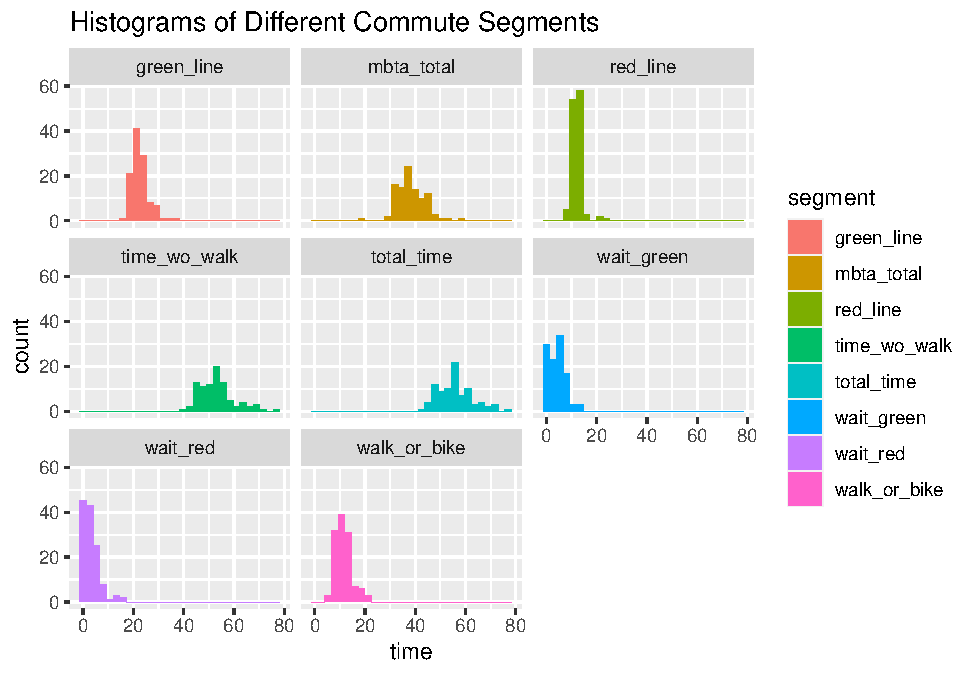
\includegraphics[width=1\linewidth]{Final_Project_Script_With_Text_files/figure-latex/unnamed-chunk-5-1} \caption{Histograms of Different Segments of the Commute}\label{fig:unnamed-chunk-5}
\end{figure}

The overall length of my commute is 55.9 minutes (nearly 56 minutes),
with a variance of 6.91 minutes. The longest segment of my commute is
the green line, which comes in at an average of 22.3 minutes and a
standard deviation of 4.08 minutes. The time it takes to travel on the
red line is 11.6 minutes, with a standard deviation of 2.12 minutes. The
waiting times for the red line and the green line are very similar: It
takes 4.05 minutes to wait for the green line, with a standard deviation
of 3.15 minutes, whereas it takes 3.18 minutes to wait for the red line,
with a standard deviation of 3.17 minutes.

Shapiro-Wilk tests for normality run across each column showed that the
data is \emph{not} normally distributed, all with p-values less than
.001. In fact, none of the segments of the dataset were normally
distributed, which is surprising because looking at the histograms, some
seem to appear bell-shaped. However, it makes sense that these segments
are not normally distributed: There is always a minimum time that it
could take the MBTA to go to different stops because time warps don't
exist yet. There is also theoretically no upper limit to how long it
might take the MBTA to arrive at its destination due to delays from
malfunctioning trains, track work, police activity, or misbehaving
passengers. Therefore, unlike with the Central Limit Theorem, the more
data collected, the more left-skewed the data will be due to outlying
delays.

\hypertarget{question-2-what-probability-distributions-can-be-used-to-model-commute-times}{%
\subsection{Question 2: What probability distributions can be used to
model commute
times?}\label{question-2-what-probability-distributions-can-be-used-to-model-commute-times}}

If we can't use normal distributions to model this data set, what can we
use? For this section of the research project, I'm going to analyze a
subset of the data displayed above. I want to model the time it takes on
the green line, the time it takes on the red line, and the time it takes
overall using maximum likelihood estimation to estimate parameters for
different distributions.

To plot these graphs, I created frequency histograms of each variable.
The optimal number of breaks in the histogram was used according to the
Freedman-Diaconis rule. To calculate the parameters of the
distributions, I used the ENVStats package which uses maximum likelihood
estimation. Several curves corresponding to different probability
distributions were plotted atop the histogram.

\hypertarget{the-distribution-for-the-total-time}{%
\subsubsection{The Distribution for the Total
Time}\label{the-distribution-for-the-total-time}}

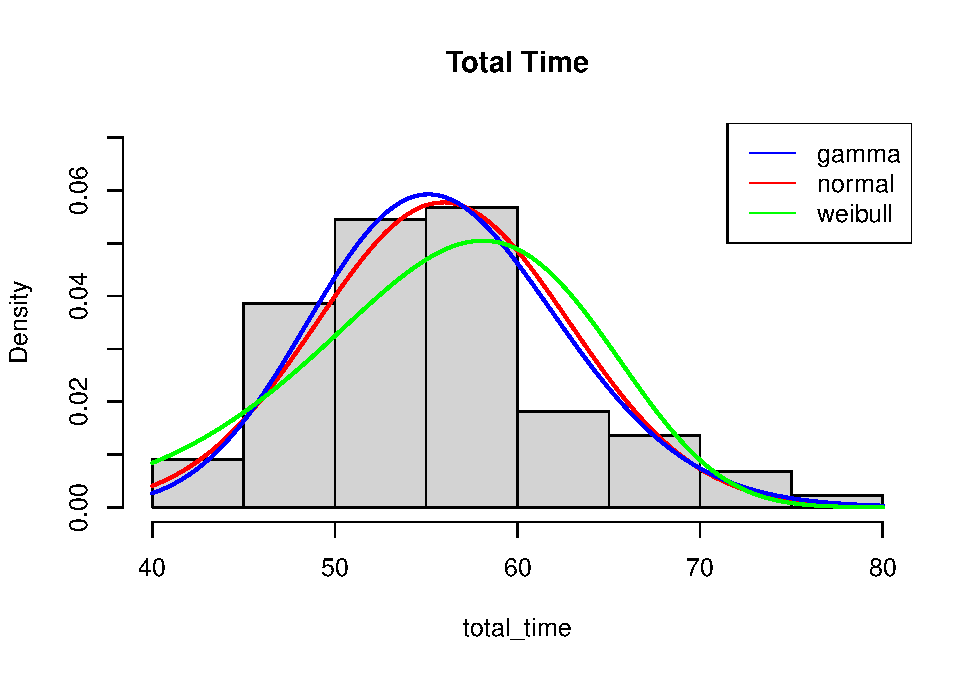
\includegraphics{Final_Project_Script_With_Text_files/figure-latex/unnamed-chunk-7-1.pdf}

Three different distributions were chosen to plot: The gamma, normal,
and weibull. Upon visual estimation, the best distribution looks like
the gamma. The gamma distribution had a shape parameter of 68.2686038
and a scale parameter of .8192905.

\hypertarget{the-distribution-for-the-green-line}{%
\subsubsection{The Distribution for the Green
Line}\label{the-distribution-for-the-green-line}}

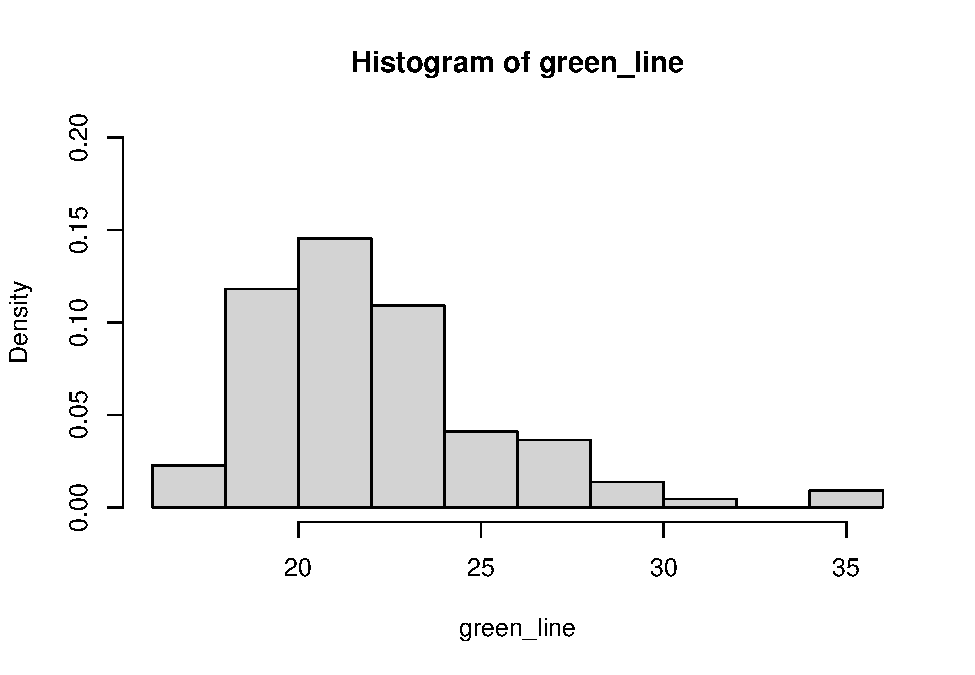
\includegraphics{Final_Project_Script_With_Text_files/figure-latex/unnamed-chunk-9-1.pdf}
\#\#\# The Distribution for the Red Line
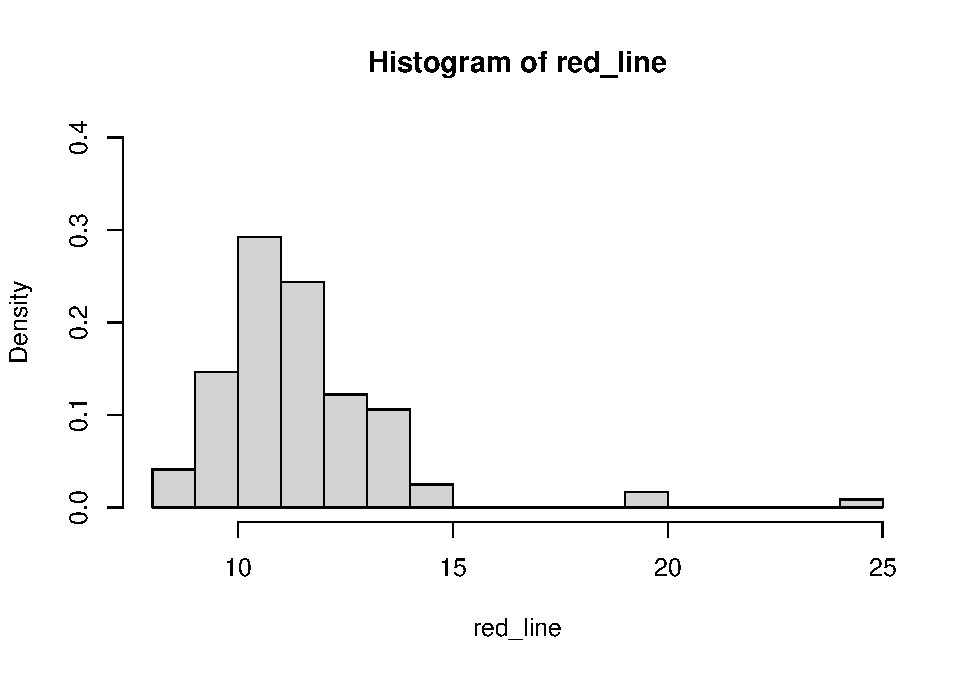
\includegraphics{Final_Project_Script_With_Text_files/figure-latex/unnamed-chunk-10-1.pdf}

\hypertarget{question-3-which-population-has-more-variance-going-to-school-in-the-morning-or-coming-home-at-night}{%
\subsection{Question 3: Which population has more variance, going to
school in the morning, or coming home at
night?}\label{question-3-which-population-has-more-variance-going-to-school-in-the-morning-or-coming-home-at-night}}

To answer this question, I subsetted my data into two vectors: the total
time it took to go home and the total time it took to come to school and
compared them using an F-test for variances, which requires populations
to be normal.

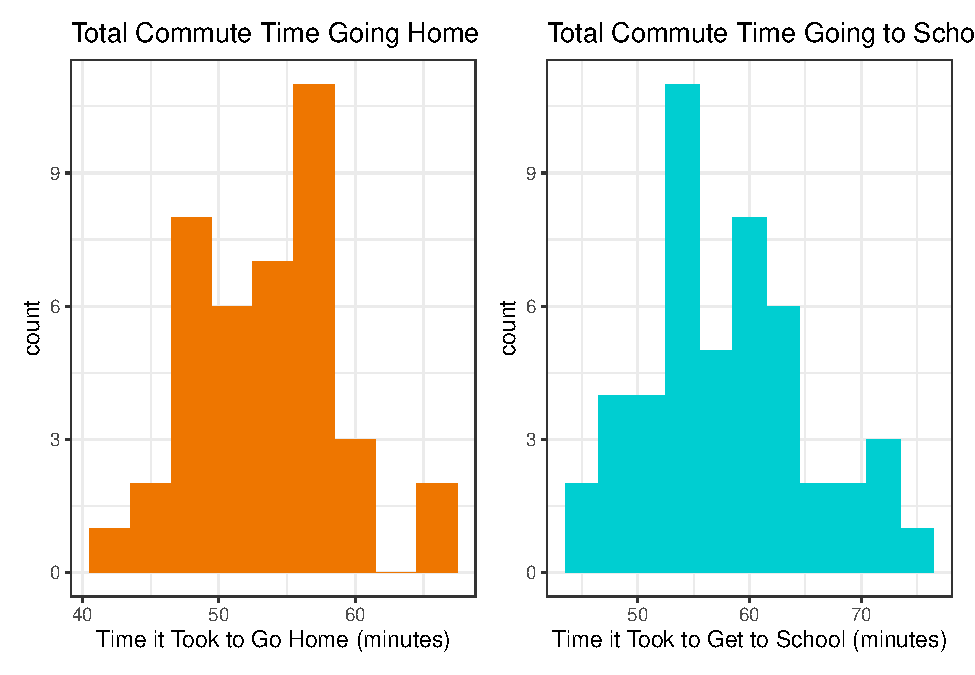
\includegraphics[width=1\linewidth]{Final_Project_Script_With_Text_files/figure-latex/unnamed-chunk-13-1}
Given that the histograms appear normal and they pass the Shapiro-Wilk
test, it is possible to then do an F-test for variances with the two
vectors.

\begin{verbatim}
## 
##  F test to compare two variances
## 
## data:  home_vector and school_vector
## F = 0.5366, num df = 39, denom df = 47, p-value = 0.04811
## alternative hypothesis: true ratio of variances is not equal to 1
## 95 percent confidence interval:
##  0.2945364 0.9947425
## sample estimates:
## ratio of variances 
##          0.5365978
\end{verbatim}

The result of the test shows a marginally significant difference between
the variation of the time it takes to come home and the time it takes to
go to school (p=.048). This is less than the widely accepted p-value of
.05, but it is very close. Looking at the data, the variance of the time
to come home is 29.0667 minutes\^{}2 and the variance of the time to go
to school is 54.1684 minutes\^{}2. Therefore, the spread in the time it
takes to go to school is slightly larger than the spread in the time it
takes to come home, although the difference is marginally significant.

This result is actually justifiable based on my commute patterns.
Previous data collection has shown that there is a significant
difference between commuting at rush hour and commuting at non-rush hour
times: Commutig at rush hour is longer and has a larger variance
compared to commuting in non rush hour times. Much of the data I took
coming home was \emph{not} during rush hour because it was at 7 or 8
p.m. Contrarily, much of the data I took going to school was
\emph{during} rush hour because it was at 8 or 9 a.m. Therefore, the
effect of rush hour may explain this result.

\hypertarget{question-4-which-segments-of-my-commute-contribute-the-most-to-its-overall-length}{%
\subsection{Question 4: Which segments of my commute contribute the most
to its overall
length?}\label{question-4-which-segments-of-my-commute-contribute-the-most-to-its-overall-length}}

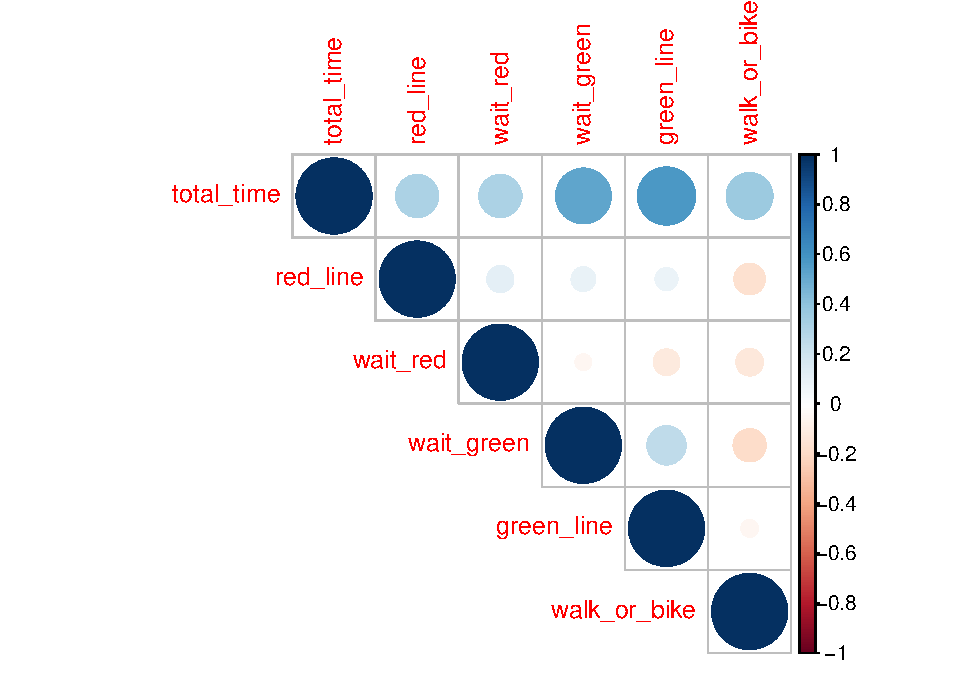
\includegraphics{Final_Project_Script_With_Text_files/figure-latex/unnamed-chunk-15-1.pdf}
Looking at the correlation plot values for total\_time, we can see that
the two darkest blues (and therefore the most positively correlated) are
how long it took to wait for the green line and how long that ride on
the green line was.

This result makes sense, as the green line is the largest and therefore
most significant part of my commute in terms of time taken up. It also
has the standard deviation of all of the individual commute segments
(i.e., commute segments that are not composites of the other segments.)
Riders of the green line know how unreliable and spotty the service can
be, especially in the part of the route that is above ground, and are
often beleaguered by delays and the trains' inability to pass each other
if one is stuck - now we have statistical evidence pointing to
unreliability!

The segments of the commute with negative correlations also have an easy
real-life explanation: If the wait for the green and red line was
longer, then the time to get from the station to the school (\emph{walk
or bike}) is shorter because it means the commute was delayed and I had
to make up for it to not be late by taking the shuttle, which is faster,
although a less eco-friendly option. Therefore, a change in behavior
(driven by not wanting to be late to class) impacted this data. One of
my original ideas was to compare two samples of being delayed versus not
being delayed to class. This did not work though because I was not late
enough times (n\textasciitilde30) during the period of the data
collection.

Surprising results in this correlation matrix include the fact that
there is a very slight negative correlation between the time waiting for
the red line versus the time waiting for the green line. The fact that
if I spend more time waiting for the green line, I spend less time
waiting for the red line later does not make sense given my limted
understanding of MBTA timetables. However, I created a linear model of
the two variables and the subsequent 99\% confidence interval of the
true slope included 0, so there is likely absolutely no measurable
correlation between those two factors and the result is only due to
random sampling.

I used the correlation matrix to identify which variables are the most
positively correlated with the overall length of the commute.

\hypertarget{linear-modelling-for-the-green-line-time}{%
\subsubsection{Linear Modelling for the Green Line
Time}\label{linear-modelling-for-the-green-line-time}}

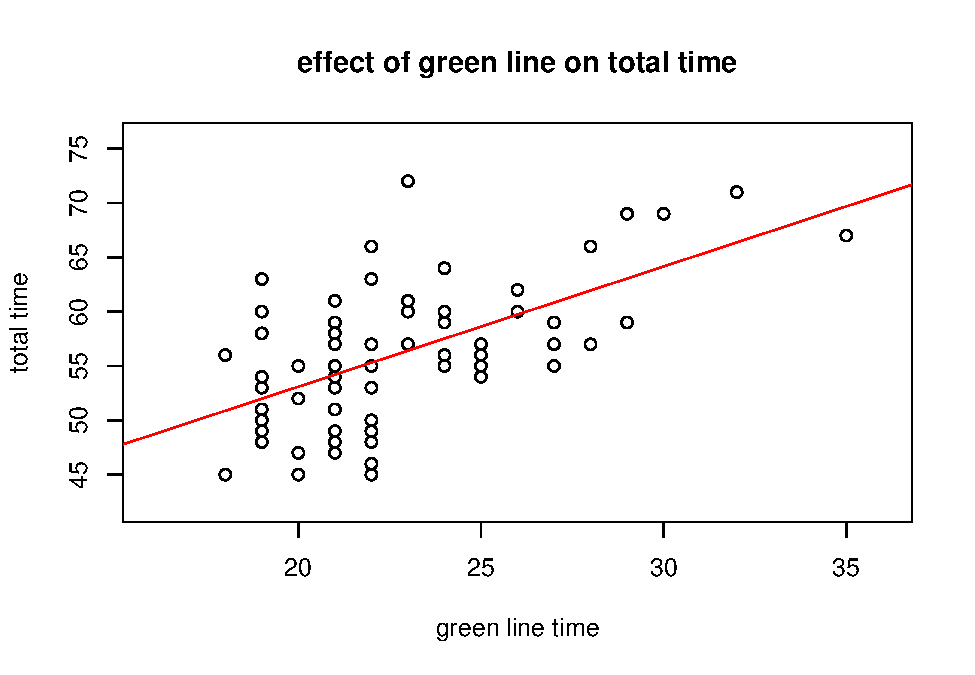
\includegraphics{Final_Project_Script_With_Text_files/figure-latex/unnamed-chunk-17-1.pdf}
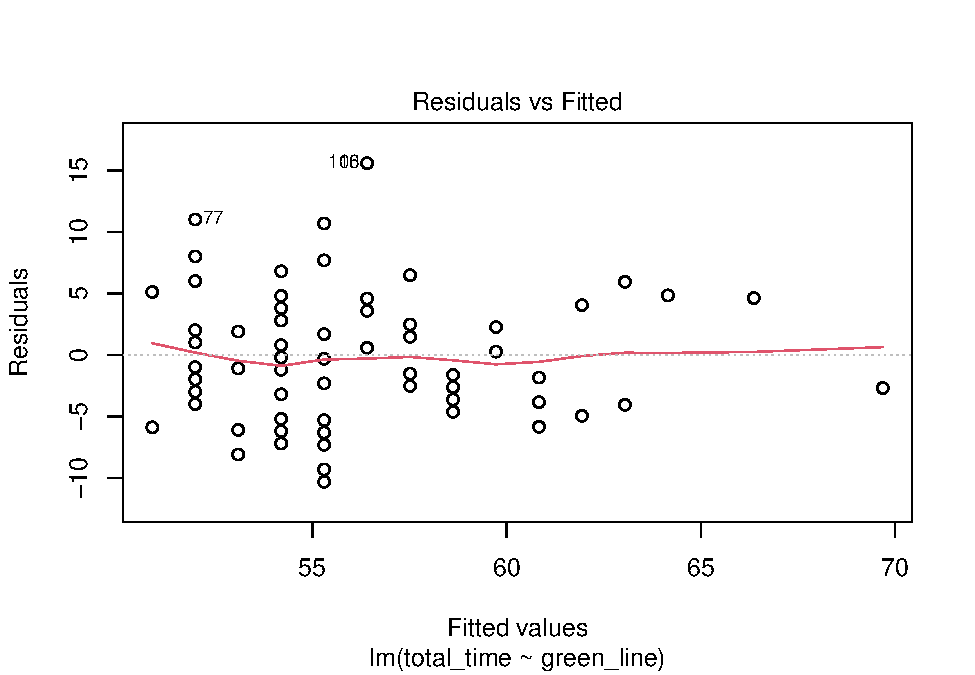
\includegraphics{Final_Project_Script_With_Text_files/figure-latex/unnamed-chunk-17-2.pdf}
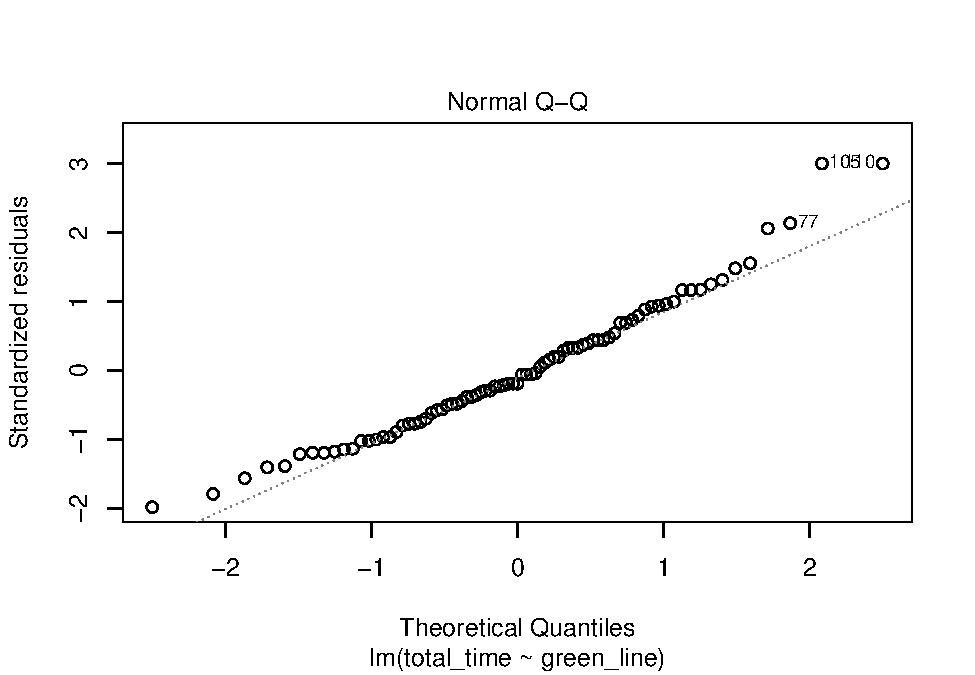
\includegraphics{Final_Project_Script_With_Text_files/figure-latex/unnamed-chunk-17-3.pdf}

\begin{verbatim}
## 
## Call:
## lm(formula = total_time ~ green_line, data = commute_2)
## 
## Residuals:
##      Min       1Q   Median       3Q      Max 
## -10.3022  -3.8334  -0.9835   2.8041  15.5916 
## 
## Coefficients:
##             Estimate Std. Error t value Pr(>|t|)    
## (Intercept)  30.9650     3.9630   7.813 2.01e-11 ***
## green_line    1.1062     0.1731   6.389 1.07e-08 ***
## ---
## Signif. codes:  0 '***' 0.001 '**' 0.01 '*' 0.05 '.' 0.1 ' ' 1
## 
## Residual standard error: 5.225 on 79 degrees of freedom
##   (77 observations deleted due to missingness)
## Multiple R-squared:  0.3407, Adjusted R-squared:  0.3323 
## F-statistic: 40.82 on 1 and 79 DF,  p-value: 1.071e-08
\end{verbatim}

In this plot, we can see that the estimated relationship between the two
variables is positive and fairly linear. The residual plot is mostly
straight and the qq-plot has a straight middle, which is good. P-values
for both the slope and the intercept are significant meaning that there
\emph{is} a statistically significant relationship between the two
variables that isn't just random or zero. The relationship between the
two variables is as follows:
\(total\)\(time = 1.1062(greenline) + 30.965\). This can be interpreted
as that if there was no green line travel at all, we could expect the
commute to be around 30 minutes. In addition, for every additional
minute on the green line, we do not spend just one more minute commuting
overall - we actually spend 1.106 minutes more. However, a 99\%
confidence interval produced did include 1, so this was likely due to
randomness. Lastly, the \(R^2\) value of .3323 means that 33.23\% of the
variance in the data set is explained by the linear model. This is a
fairly decent model which shows the effects of the green line on the
overall time.

\hypertarget{linear-modelling-for-the-time-spent-waiting-for-the-green-line}{%
\subsubsection{Linear Modelling for the Time Spent Waiting for the Green
Line}\label{linear-modelling-for-the-time-spent-waiting-for-the-green-line}}

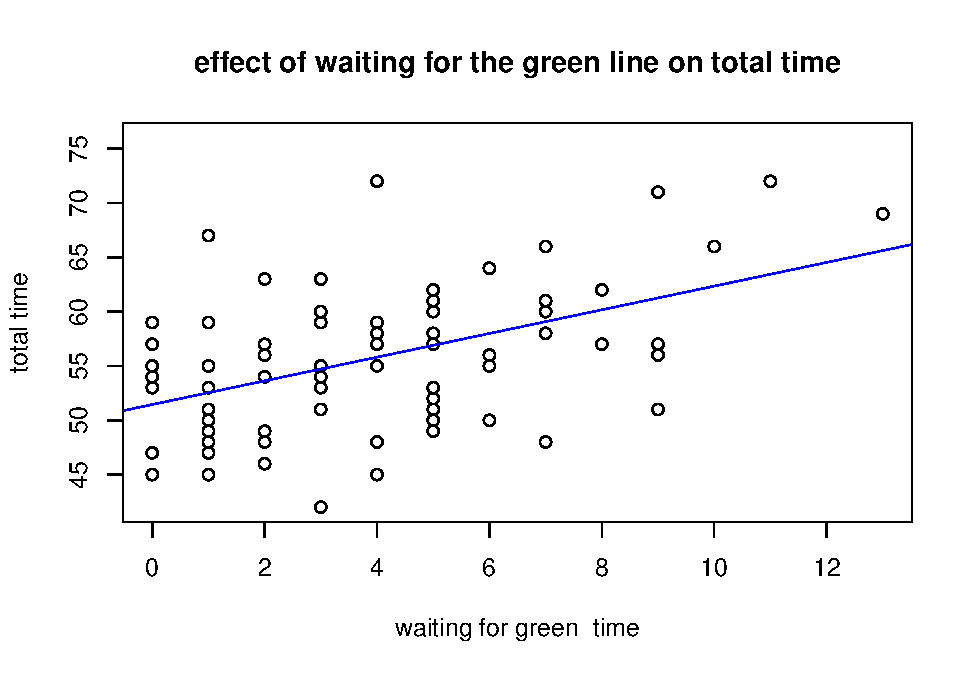
\includegraphics{Final_Project_Script_With_Text_files/figure-latex/unnamed-chunk-18-1.pdf}
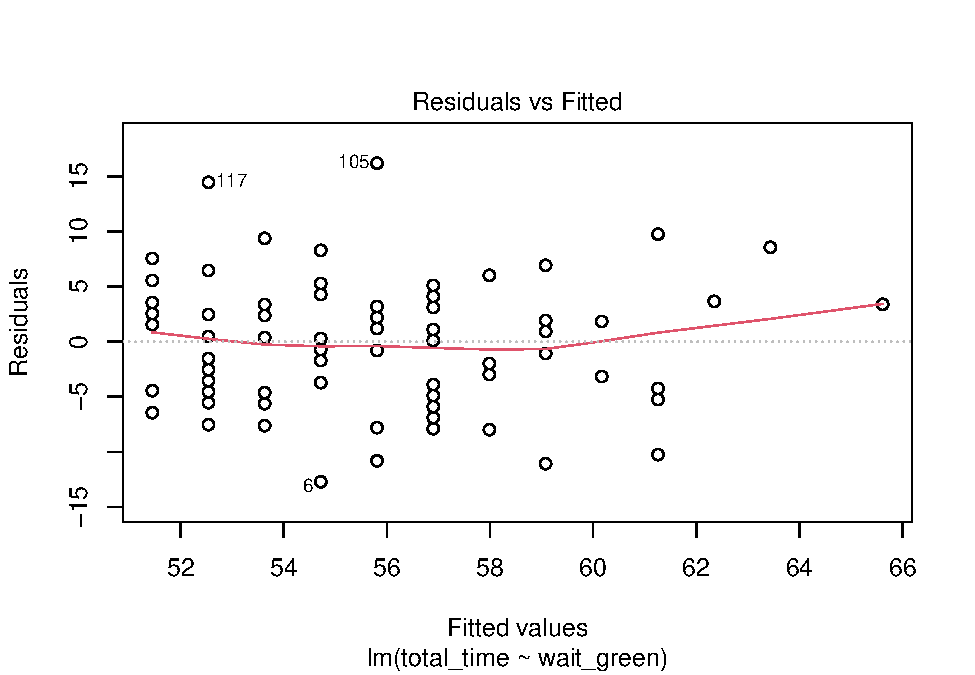
\includegraphics{Final_Project_Script_With_Text_files/figure-latex/unnamed-chunk-18-2.pdf}
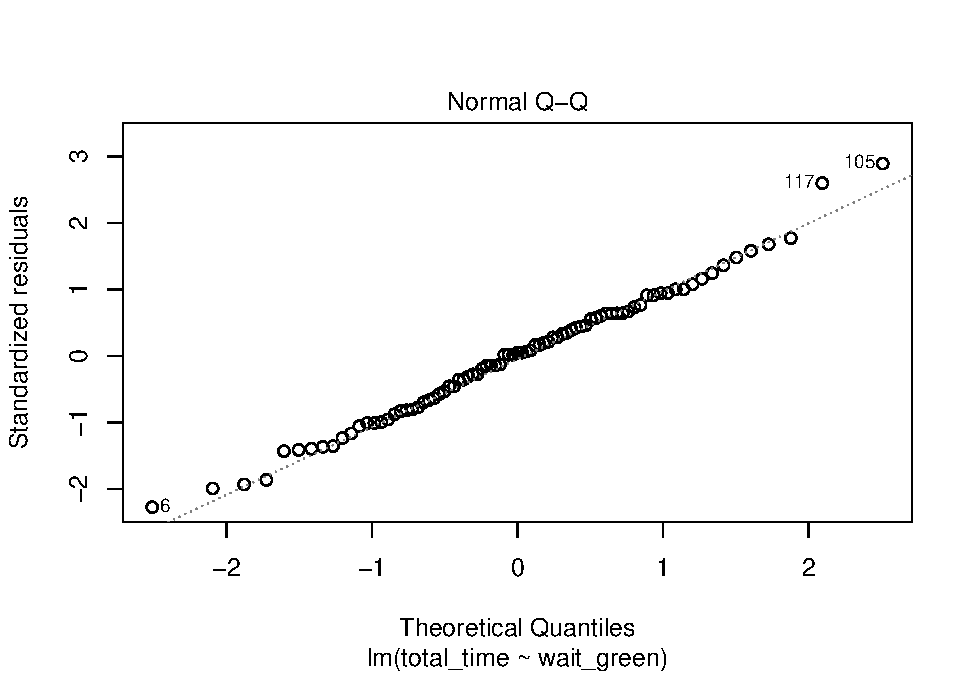
\includegraphics{Final_Project_Script_With_Text_files/figure-latex/unnamed-chunk-18-3.pdf}

\begin{verbatim}
## 
## Call:
## lm(formula = total_time ~ wait_green, data = commute_2)
## 
## Residuals:
##      Min       1Q   Median       3Q      Max 
## -12.7197  -4.0785   0.2803   3.4663  16.1906 
## 
## Coefficients:
##             Estimate Std. Error t value Pr(>|t|)    
## (Intercept)  51.4505     1.0136  50.762  < 2e-16 ***
## wait_green    1.0897     0.2021   5.392 6.71e-07 ***
## ---
## Signif. codes:  0 '***' 0.001 '**' 0.01 '*' 0.05 '.' 0.1 ' ' 1
## 
## Residual standard error: 5.629 on 81 degrees of freedom
##   (75 observations deleted due to missingness)
## Multiple R-squared:  0.2642, Adjusted R-squared:  0.2551 
## F-statistic: 29.08 on 1 and 81 DF,  p-value: 6.707e-07
\end{verbatim}

Again, we can see that the relationship between the two variables is
positive and fairly linear. The residual plot is mostly straight and the
qq-plot has a straight middle, which is good. Again, P-values for both
the slope and the intercept are significant meaning that there \emph{is}
a statistically significant relationship between the two variables that
isn't just random or zero.

The relationship between the two variables is as follows:
\(total\)\(time = 1.0897(waitgreen) + 51.4505\). This can be interpreted
as that if there was no waiting for the green line at all, we could
expect the commute to be around 51 minutes and 30 seconds. In addition,
for every additional minute waiting for the green line, we do not spend
just one more minute commuting overall - we actually spend 1.0897
minutes more. However, this is not significantly different than 1, as
the 99\% confidence interval produced for the slope did include 1.
Lastly, the \(R^2\) value of .2551 means that around 25\% of the
variance in the data set is explained by the linear model. Therefore,
this model shows that the driving force behind the overall length of the
commute may not be the time it takes to wait for the green line.

\hypertarget{question-5-how-long-can-i-expect-my-commute-to-be}{%
\subsection{Question 5: How long can I expect my commute to
be?}\label{question-5-how-long-can-i-expect-my-commute-to-be}}

\hypertarget{conclusions-limitations}{%
\section{Conclusions \& Limitations}\label{conclusions-limitations}}

In conclusion, my commute takes \emph{way} too long. Important things we
learned in the study include: MORE HERE.

This study, as with all studies, has its limitations. Firstly, the data
was collected by me in a convenience sample so there was a lot of
potential bias and systematic errors. In order to have a true
representation of the mean time it takes to commute, these times should
have been evenly distributed across the hours and days of the week. The
data was collected only to the minute so the precision is low,
especially because during rush hour, being a few seconds later can
result in a person missing the first train and having to wait another
fifteen minutes (not like I speak from experience). Therefore, further
studies about my commute should involve stochasticity. Precision by
using a smart watch with the seconds synced to a world clock could also
be implemented in future studies. Lastly, another direction I would like
to take this project in is comparing my own time to the estimated times
given by the countdown clocks in the stations and apps such as
\href{https://transitapp.com/}{Transit}, which is the only app to be
endorsed by the MBTA
\href{https://www.wbur.org/bostonomix/2016/09/06/mbta-best-transit-app}{officially}.

\hypertarget{citations-packages-used}{%
\subsection{Citations \& Packages Used}\label{citations-packages-used}}

Owen, W. J., \& Wackerly, D. D. (2008). \emph{Mathematical statistics
with applications, seventh edition, Dennis Wackerly, William Mendenhall,
Richard L. Scheaffer.} Belmont, CA: Brooks/Cole Cengage Learning.

R Core Team (2020). R: A language and environment for statistical
computing. R Foundation for Statistical Computing, Vienna, Austria. URL
\url{https://www.R-project.org/}.

Taiyun Wei and Viliam Simko (2017). R package ``corrplot'':
Visualization of a Correlation Matrix (Version 0.84). Available from
\url{https://github.com/taiyun/corrplot}

Thomas Lin Pedersen (2019). patchwork: The Composer of Plots. R package
version 1.0.0. \url{https://CRAN.R-project.org/package=patchwork}

Wickham et al., (2019). Welcome to the tidyverse. Journal of Open Source
Software, 4(43), 1686, \url{https://doi.org/10.21105/joss.01686}

Millard SP (2013). \emph{EnvStats: An R Package for Environmental
Statistics}. Springer, New York. ISBN 978-1-4614-8455-4, \textless URL:
\url{http://www.springer.com}\textgreater.

Yihui Xie (2020). knitr: A General-Purpose Package for Dynamic Report
Generation in R. R package version 1.28.

\end{document}
